\section{Level Crossing and Balance Equations}
\label{sec:level-cross-balance}



\opt{solutionfiles}{
\subsection*{Theory and Exercises}
\Opensolutionfile{hint}
\Opensolutionfile{ans}
}

Consider a system at which customers arrive and depart in single entities, such as customers in a shop or jobs at some machine.
If the system starts empty, then we know that the number $L(t)$ in the system at time $t$ is equal to $A(t) - D(t)$.
To illustrate:

\begin{figure}[h]
  \centering
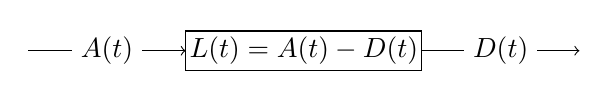
\begin{tikzpicture}[scale=1]
\draw[->] (0,0)--node[midway, fill=white] {$A(t)$}  (2,0); 
\draw (2,-0.25) rectangle node {$L(t)=A(t)-D(t)$} (5,0.25);
\draw[->] (5,0)--node[midway, fill=white] {$D(t)$}  (7,0); 
\end{tikzpicture}
\end{figure}

\noindent What goes in the box (i.e., $A(t)$) minus what has already gone out
  (i.e., $D(t)$) must still be in the box, hence $L(t)=A(t)-D(t)$. 



  Let us denote an arrival as an `up-crossing' and a departure as a `down-crossing'.
  Then, clearly $L(t)$ is the number of up-crossings up to time $t$ minus the number of down-crossings up to time $t$.
  If $L(t)$ remains finite, or, more generally, $L(t)/t \to 0$ as $t\to\infty$, then it must be that
\begin{equation*}
  \lambda =  \lim_{t \to \infty} \frac{A(t)}t  = \lim_{t \to \infty} \frac{D(t)+L(t)}t =  \lim_{t \to \infty} \frac{D(t)}t + \lim_{t \to \infty} \frac{L(t)}t 
  = \delta.  
\end{equation*}
Hence, when $L(t)/t\to0$, the \recall{up crossing rate} $\lim_{t \to \infty} A(t)/t = \lambda$ is equal to the \emph{down-crossing rate} $\lim_{t \to \infty} D(t)/t = \delta$.
We will generalize these notions of up- and downcrossing in this section to derive the \emph{stationary}, or \emph{long-run time average} or \emph{steady-state}, distribution $p(n)$ that the system contains $n$ jobs.

\begin{extra}
  If $L(t)/t \to 0$ as $t\to\infty$, can it still be true that $\E{L}>0$? 
  \begin{solution}
    \begin{equation*}
      \E{L} = \lim_{t\to\infty} \frac 1 t \int_0^t L(s) \d s \neq \lim_{t\to\infty} \frac{L(t)}t.
    \end{equation*}
If $L(t)=1$ for all $t$, $\E{L} =1 $, but $L(t)/t \to 0$. 
  \end{solution}
\end{extra}

Let us say that the system is in \emph{state $n$} at time $t$ when it contains $n$ jobs at that moment, i.e., when $L(t) = n$.
The system \emph{crosses} level $n$ at time $t$ when its state changes from $n$ to $n+1$, either `from below' due to an arrival, or `from above' due to a departure, cf.~\cref{fig:A_n_t}.

\begin{figure}[th]
  \centering
\begin{tikzpicture}[scale=1,->,>=stealth',shorten >=1pt,auto,node distance=1.8cm,
                    semithick]
  \node[state] (0) {$p(0)$} ;
  \node[state] (1) [right of=0] {$p(1)$};
  \node[state] (2) [right of=1] {$p(2)$};
  \node[state] (3) [right of=2] {$p(3)$};
  \node[state] (4) [right of=3] {$\cdots$};

\path 
 (0) edge [bend left] node {$\lambda(0)$} (1)
 (1) edge [bend left] node {$\mu(1)$} (0)
 (1) edge [bend left] node {$\lambda(1)$} (2)
 (2) edge [bend left] node {$\mu(2)$} (1)
 (2) edge [bend left] node {$\lambda(2)$} (3)
 (3) edge [bend left] node {$\mu(3)$} (2)
 (3) edge [bend left] node {$\lambda(3)$} (4)
 (4) edge [bend left] node {$\mu(4)$} (3);

\draw[-, dotted, gray] (2.7,-2.)--(2.7,2.0) node[above, black] {level $1$};
\draw[->] (2,1.5)  node[left] {$A(1,t)$} -- (3.5,1.5);
\draw[<-] (2,-1.2) node[left] {$D(1,t)$} --(3.5,-1.2) ;

\end{tikzpicture}
\caption{ $A(1,t)$ counts the number of jobs up to time $t$ that saw 1
  job in the system upon arrival, and right after such arrivals the
  system contains 2 jobs.  Thus, each time $A(1,t)$ increases by
  one, level $1$ (the dotted line  separating states 1 and 2) is crossed from below.  Similarly, $D(1,t)$ counts the number of
  departures that leave 1 job behind, and just before such departures the system contains 2 jobs. Hence, level $1$ is crossed from above. 
It is evident that the number of times this
  level is crossed from below must be the same (plus or minus 1) the
  number of times it is crossed from above. (We introduce $\lambda(n)$, $\mu(n)$ and $p(n)$ below.) }
\label{fig:A_n_t}
\end{figure}


To establish the section's main result~\cref{eq:12} we need a few definitions that are quite subtle and might seem a bit abstract, but below we will provide intuitive interpretations in terms of system KPIs.
Once we have the proper definitions, the above result will follow straightaway.
\Cref{fig:summaries} at the end of the section summarizes all concepts we develop here.

\paragraph{Level crossing}




Define
\begin{subequations}\label{eq:rates_}
\begin{equation}\label{eq:19} 
  A(n,t) = \sum_{k=1}^\infty \1{A_k \leq t}\1{L(A_k-) = n}
\end{equation}
as the number of arrivals up to time $t$ that saw $n$ customers in the system at their arrival.

\begin{extra}
  Why do we  take $L(A_k-)=n$ rather than $L(A_k)$ in the definition of $A(n,t)$?
  \begin{hint}
Recall that $L(t)$ is \emph{right-continuous}.
  \end{hint}
    \begin{solution}
      $L(t)$ is the number of customers in the system at time $t$.
      As such the function $t\to L(t)$ is \textsl{right-continuous}.
      The definition of $L(A_k-) = \lim_{t\uparrow A_k} L(t)$ is the limit from the left.
      The customer therefore `sees' $L(A_k-)$ just before he/she arrives.
\end{solution}  
\end{extra}

\begin{extra}\label{ex:36}
If   $A(n,t) = \sum_{k=1}^\infty \1{A_k \leq t}\1{L(A_k-) = n}$, is  $A(t) =\sum_{n=0}^\infty A(n,t)$?
\begin{solution}
  $A(t)$ counts all customers that arrive up to time $t$, i.e., during
  $[0,t]$. Note that this \textsl{includes} time $t$. $A(n,t)$ counts
  the jobs that see $n$ jobs in the system just before they arrive. As there either $0$, or $1$, or $2$, etc., jobs in the system upon arrival the summation covers all possible outcomes. Therefore the claim is true. 
    \end{solution}
\end{extra}

\begin{extra}
 Show that $A(n,t) \leq A(t)$. 
\begin{solution}
       Observe that
      $\1{A_k\leq t}\1{L(A_k-) = n} \leq \1{A_k\leq t}$;
      the last inequality follows from the fact that
      $\1{L(A_k-) = n}\leq 1$. Therefore,
    \begin{equation*}
  A(n,t) = \sum_{k=1}^\infty \1{A_k \leq t} \1{L(A_k-) = n} 
\leq \sum_{k=1}^\infty \1{A_k \leq t} = A(t). 
    \end{equation*}
    For any `normal' queueing system, $A(t) > A(n,t)$, because the
    queue length fluctuates.
    \end{solution}
\end{extra}

\begin{extra}\label{ex:38}
If $\lambda>\delta$ it can happen that  $ \lim_{t\to\infty} A(n,t)/t > 0$ for some (finite) $n$. 
  \begin{solution}
    If $\lambda > \delta$, then $L(t)\to\infty$.
    But then there must be a last time, $s$ say, that $L(s) = n+1$, and $L(t) > n+1$ for all $t>s$.
    Hence, after time $s$ no job will see the system with $n$ jobs.
    Thus $A(n,t) = A(n,s)$ for all $t>s$.
    This is a finite number, while $t\to\infty$, so that $A(n,t)/t \to 0$.
  \end{solution}
\end{extra}


Next, let 
\begin{equation} \label{eq:17} 
   Y(n,t) = \int_0^t  \1{L(s) = n} \d s
\end{equation}
be  the total time the system contains $n$ jobs during $[0,t]$, and
\begin{equation} \label{eq:18}
   p(n,t) = \frac 1 t \int_0^t  \1{L(s) = n} \d s = \frac{Y(n,t)}t,
\end{equation}
\end{subequations}
be the fraction of time that $L(s) =n$ in $[0,t]$. ~\Cref{fig:Y_1_t} illustrates the relation between $Y(n,t)$ and $A(n,t)$.
  
 \begin{exercise} \label{ex:111} Consider the following (silly) queueing process.
   At times $0, 2,4, \ldots$ customers arrive, each customer requires $1$ unit of service, and there is one server.
   Find an expression for $A(n,t)$.
   (What acronym would describe this queueing situation?)
  \begin{hint}
    For the acronym, observe that the service times and inter-arrival are deterministic and there is one server.
    For the computation of $Y(n,t)$, make a plot of $L(s)$ as a function of time for $n=1$.

    Make a plot of $L(s)$ for $n=1$ as a function of time.
  \end{hint}
    \begin{solution}
      It is the $D/D/1$ queue, since there is one server and the inter-arrival times and service times are constant, i.e., deterministic.
      $A_k = 2k$ as jobs arrive at $t=0, 2, 4, \ldots$, hence, $A(t) \approx t/2$ when $t\gg 0$.
      We also know that $L(s)=1$ if $s\in [2i, 2i+1)$ and $L(s)=0$ for $s\in[2i-1, 2i)$ for $i=0, 1, 2, \ldots$.
      Thus, $L(A_k-) = L(2k-)=0$.
      Hence, $A(0,t) \approx t/2$ for $t\gg 0$, and $A(n,t)=0$ for $n\geq 1$.
    \end{solution}
\end{exercise}


\begin{exercise}[Continuation of~\ref{ex:111}] \label{ex:112} 
  Find an expression for $Y(n,t)$.
    \begin{solution}
      Next, to get $Y(n,t)$, observe that the system never contains
      more than 1 job. Hence, $Y(n,t)=0$ for all $n\geq 2$.  Then we see that
      $Y(1,t) = \int_0^t \1{L(s) = 1}\d s.$ Now observe that for our
      queueing system $L(s)=1$ for $s\in[0,1)$, $L(s)=0$ for
      $s\in[1,2)$, $L(s)=1$ for $s\in[2,3)$, and so on. Thus, when
      $t<1$, $Y(1,t)=\int_0^t \1{L(s)=1} \d s = \int_0^t 1\d s = t$.
      When $t\in[1,2)$, 
      \begin{equation*}
        L(t)=0 \implies \1{L(t)=0} \implies Y(1,t) \text{ does not change}.
      \end{equation*}
Continuing to $[2,3)$ and so on gives
    \begin{equation*}
      Y(1,t) =
      \begin{cases}
        t & t\in[0,1), \\
        1 & t\in[1,2), \\
        1+(t-2) & t\in[2,3), \\
        2 & t\in[3,4), \\
        2+(t-4) & t\in[4,5), \\
      \end{cases}
    \end{equation*}
    and so on.  Since $Y(n,t)=0$ for all $n\geq 2$, $L(s) = 1$ or
    $L(s)=0$ for all $s$, therefore, 
    \begin{equation*}
      Y(0,t) = t-Y(1,t).
    \end{equation*}
    \end{solution}
\end{exercise}


\begin{figure}[t]
  \centering
\begin{tikzpicture}[scale=1,
  open/.style={shape=circle, fill=white, inner sep=1pt, draw, node contents=},
  closed/.style={shape=circle, fill=black, inner sep=1pt, draw, node contents=},
]

%axis
\draw[->] (0,0) -- coordinate (x axis mid) (8.5,0);
\draw[->] (0,0) -- coordinate (y axis mid) (0,4.5);
%\node[below=0.2cm] at (x axis mid) {$t$};
\node[left=0.3cm, rotate=90] at (y axis mid) {$L(t)$};


\draw 
node (0) at (0,0) [closed] {}
node (c1) at (1,0) [open] {};
\draw[thick] (0)--(c1);
\node[below] at (1,0) {$A_1$};

\draw 
node (c2) at (1,1) [closed] {}
node (c3) at (2.5,1) [open] {};
\draw[thick] (c2)--(c3);
\node[below] at (2.5,0) {$D_1$};

\draw 
node (c2) at (2.5,0) [closed] {}
node (c3) at (3,0) [open] {};
\draw[thick] (c2)--(c3);
\node[below] at (3,0) {$A_2$};

\draw 
node (c2) at (3,1) [closed] {}
node (c3) at (4,1) [open] {};
\draw[thick] (c2)--(c3);

\draw 
node (c2) at (4,2) [closed] {}
node (c3) at (5,2) [open] {};
\draw[thick] (c2)--(c3);
\node[below] at (4,0) {$A_3$};

\draw 
node (c2) at (5,1) [closed] {}
node (c3) at (5.8,1) [open] {};
\draw[thick] (c2)--(c3);
\node[below] at (5.,0) {$D_2$};

\draw 
node (c2) at (5.8,2) [closed] {}
node (c3) at (6.3,2)  {};
\draw[thick] (c2)--(c3);
\node[below] at (5.8,0) {$A_4$};

\draw[dashed] (1,0)--(2.5, 1.5) -- (3, 1.5)--(4,2.5) -- 
(5, 2.5)--(5.8, 3.3)--(6.3, 3.3);
\node[right] at (6.3, 3.3) {$Y(1,t)$};

\draw[dotted] (4,0) -- (4,0.5)--(5.8, 0.5)--(5.8, 1.5)--(6.3, 1.5);
\node[right] at (6.3, 1.5) {$A(1,t)$};

\end{tikzpicture}
  \caption{Plots of $Y(1,t)$ and $A(1,t)$. (For visual clarity, we subtracted $1/2$ from $A(1,t)$, for otherwise its graph would partly overlap with the graph of $L$.)}
  \label{fig:Y_1_t}
\end{figure}



Define also the limits:
\begin{align}\label{eq:p(n)}
  \lambda(n) &= \lim_{t\to\infty} \frac{A(n,t)}{Y(n,t)}, &p(n) &=\lim_{t\to\infty} p(n,t),
\end{align}
as the \emph{arrival rate in state $n$} and the \emph{long-run fraction of
  time the system spends in state $n$}. To clarify the former
definition, observe that $A(n,t)$ counts the number of arrivals that
see $n$ jobs in the system upon arrival, while $Y(n,t)$ tracks the amount of time
the system contains $n$ jobs. Suppose that at time~$T$ a job arrives that
sees $n$ jobs in the system. Then $A(n,T)=A(n, T-)+1$, and this job finishes
an interval that is tracked by $Y(n,t)$, precisely because this job
sees $n$ jobs in the system just prior to its arrival. Thus, just as
$A(t)/t$ is the total number of arrivals during $[0,t]$ divided by~$t$, $A(n,t)/Y(n,t)$ is the number of arrivals that see $n$ jobs divided by
the time the system contains $n$ jobs.

\begin{exercise}[Continuation of \ref{ex:112}] \label{ex:113} Compute $p(n)$ and $\lambda(n)$.
  \begin{solution}
    From the other exercises:
    \begin{align*}
      \lambda(0) &\approx \frac{A(0,t)}{Y(0,t)} \approx \frac{t/2}{t/2} = 1, \\
      \lambda(1) &\approx \frac{A(1,t)}{Y(1,t)} \approx \frac{0}{t/2} = 0, \\
      p(0) &\approx \frac{Y(0,t)}{t} \approx \frac{t/2}{t} = \frac 1 2, \\
      p(1) &\approx \frac{Y(1,t)}{t} \approx \frac{t/2}{t} = \frac 1 2.
    \end{align*}
For the rest $\lambda(n) = 0$, and $p(n)=0$, for $n\geq 2$.
  \end{solution}
\end{exercise}

Similar to the definition for $A(n,t)$, let
\begin{equation*}
    D(n,t) = \sum_{k=1}^\infty \1{D_k \leq t} \1{L(D_k) = n}
  \end{equation*}
  denote the number of departures up to time $t$ that\emph{ leave $n$
    customers behind}. Then,  define
\begin{equation*}
  \mu(n+1) = \lim_{t\to\infty} \frac{D(n,t)}{Y(n+1,t)},
\end{equation*}
as \emph{ the departure rate from state $n+1$}.
(It is easy to get confused here: to leave $n$ jobs behind, the system must contain $n+1$ jobs just prior to the departure.)
\Cref{fig:A_n_t} shows how $A(n,t)$ and~$\lambda(n)$ relate to $D(n+1,t)$ and $\mu(n)$.

\begin{extra}\label{ex:39}
Should  we take $D(n-1,t)$ or  $D(n,t)$ in the definition of $\mu(n)$?
    \begin{solution}
      $D(n-1,t)$ counts the departures that leave $n-1$ behind. Thus,
      just before the customer leaves, the system contains $n$
      customers.
\end{solution}
\end{extra}

\begin{exercise}[Continuation of~\ref{ex:113}] \label{ex:4}
Compute 
$D(n,t)$ and $\mu(n+1)$ for $n\geq 0$.
\begin{solution}
  $D(0,t) = \sum_{k=1}^\infty\1{D_k\leq t, L(D_k)=0}$. From the graph of $\{L(s)\}$ we see that all jobs leave an empty system behind. Thus, $D(0,t) \approx t/2$, and $D(n,t)=0$ for $n\geq 1$. With this, $D(0,t)/Y(1,t) \sim (t/2)/(t/2) = 1$, and so,
  \begin{equation*}
    \mu(1) = \lim_{t\to\infty} \frac{D(0,t)}{Y(1, t)} = 1,
  \end{equation*}
and $\mu(n) = 0$ for $n\geq2$. 
\end{solution}
\end{exercise}

Observe that customers arrive and depart as single units. Thus, if
$\{T_k\}$ is the ordered set of arrival and departure times of the
customers, then $L(T_k) = L(T_k-) \pm 1$. But then we must also have
that $|A(n,t) - D(n,t)| \leq 1$ (think about this). From this
observation it follows immediately that
\begin{equation}\label{eq:15}
  \lim_{t\to\infty} \frac{A(n,t)}t = \lim_{t\to\infty} \frac{D(n,t)}t.
\end{equation}
With this equation we can obtain two nice and fundamental
identities. The first we develop now; the second follows in~\cref{sec:poisson-arrivals-see}.

The rate of jobs that `see the system with $n$ jobs' can be defined as
$A(n,t)/t$. Taking limits we get
\begin{subequations}
\label{eq:21}
\begin{equation}\label{eq:63}
\lim_{t\to\infty}  \frac{A(n,t)}t =  \lim_{t\to\infty} \frac{A(n,t)}{Y(n,t)}\frac{Y(n,t)}t = \lambda(n) p(n),
\end{equation}
where we use the above definitions for $\lambda(n)$ and $p(n)$.
Similarly, the departure rate of jobs that leave $n$ jobs behind is
\begin{equation}\label{eq:22}
\lim_{t\to\infty}  \frac{D(n,t)}t =  \lim_{t\to\infty} \frac{D(n,t)}{Y(n+1,t)}\frac{Y(n+1,t)}t = \mu(n+1) p(n+1).
\end{equation}
\end{subequations}
Combining this with~\cref{eq:15} we arrive at the \recall{level crossing equations}
\begin{equation}\label{eq:12}
  \lambda(n) p(n) = \mu(n+1)p(n+1).
\end{equation}

\begin{exercise}[Continuation of~\ref{ex:4}] Compute $\lambda(n) p(n)$ for $n\geq 0$, and check $\lambda(n) p(n) = \mu(n+1) p(n+1)$.
\begin{solution}
  $\lambda(0)p(0)=1\cdot 1/2 = 1/2$, $\lambda(n)p(n)= 0$ for $n>1$, as $\lambda(n)=0$ for $n>0$.

From Exercise~\ref{ex:4}, $\mu(1)=1$, hence $\mu(1) p(1) = 1\cdot 1/2 = 1/2$. Moreover, $\mu(n)=0$ for $n\geq 2$. 

Clearly, for all $n$ we have $\lambda(n)p(n)= \mu(n+1)p(n+1)$. 

\end{solution}
\end{exercise}

Result~\cref{eq:12} turns out to be exceedingly useful, as will become evident from~\cref{sec:mm1} onward.
More specifically, by specifying (i.e., modeling) $\lambda(n)$ and $\mu(n)$, we can compute the long-run fraction of time $p(n)$ that the system contains $n$ jobs.
To see this, rewrite the above into
\begin{equation}\label{eq:25}
  p(n+1) = \frac{\lambda(n)}{\mu(n+1)}p(n). 
\end{equation}
Thus, this equation fixes the ratios between the probabilities. In other words, if we know $p(n)$ we can compute $p(n+1)$, and so on. Hence, if $p(0)$ is known, then $p(1)$ follows, from which $p(2)$
follows, and so on. A straightaway iteration then leads to
\begin{equation}\label{eq:38}
  p(n+1) = \frac{\lambda(n)\lambda(n-1)\cdots \lambda(0)}{\mu(n+1)\mu(n)\cdots \mu(1)}p(0).
\end{equation}

To determine $p(0)$ we can use the fact that the numbers $p(n)$ represent probabilities.
Hence, from the normalizing condition $\sum_{n=0}^\infty p(n)=1$, we get $p(0) = G^{-1}$ with
% \begin{align*}
% 1 
% &= \sum_{n=0}^\infty p(n) \\
% &= p(0) \left(1+\sum_{n=0}^\infty \frac{\lambda(n)\lambda(n-1)\cdots\lambda(0)}{\mu(n+1)\mu(n)\cdots \mu(1)}\right),
% \end{align*}
% we obtain  
$G$ being the \recall{normalization constant}
\begin{equation}
  \label{eq:20}
G = 1+\sum_{n=0}^\infty \frac{\lambda(n)\lambda(n-1)\cdots\lambda(0)}{\mu(n+1)\mu(n)\cdots \mu(1)}.
\end{equation}

In the next few sections we will make suitable choices for $\lambda(n)$ and $\mu(n)$ to model many different queueing situations so that, based on \cref{eq:12}, we can obtain simple expressions for $p(n)$ in terms of the arrival and service rates.
With $p(n)$ we define  two easy, but important performance measures. The time-average average number of items becomes
\begin{equation*}
\E L = \sum_{n=0}^\infty n p(n),
\end{equation*}
and the long-run fraction of time the system contains at least $n$ jobs is
\begin{equation*}
  \P{ L \geq n} = \sum_{i=n}^\infty p(i).
\end{equation*}

\begin{exercise}
  Derive  $\E L = \sum_{n=0}^\infty n p(n)$ from~\cref{eq:46}. 
\begin{solution}
As $L(s)$ counts the number of jobs in the system at time $s$ (thus $L(s)$ is an integer),
\begin{equation*}
  L(s) = \sum_{n=0}^\infty n\, \1{L(s) = n}.
\end{equation*}
With this we can write for the time-average number of jobs in the system
\begin{equation}\label{eq:1}
\frac 1 t \int_0^t L(s) \d s = \frac 1 t \int_0^t \left(\sum_{n=0}^{\infty} n\, \1{L(s) = n}\right) \d s
= \sum_{n=0}^{\infty} \frac n t \int_0^t   \1{L(s) = n} \d s,
\end{equation}
where we interchange the integral and the summation\footnote{This is allowed as the integrand is non-negative.
  More generally, the interested reader should check Fubini's theorem.}.
It then follows from~\cref{eq:18} that
\begin{equation*}
\frac 1 t \int_0^t L(s) \d s =  \sum_{n=0}^{\infty} n\, p(n,t).
\end{equation*}
Finally, assuming that the limit $p(n,t) \to p(n)$ exists as
$t\to\infty$ (and that the summation and limit can be interchanged in
the above), the result follows.
\end{solution}
\end{exercise}






Finally, the following two exercises show that level crossing arguments extend well beyond the queueing systems modeled by~\cref{fig:A_n_t}.

\begin{exercise}\label{ex:67}
Consider a single server that serves one queue and serves only in batches of 2 jobs at a time (so never 1 job or more than 2 jobs), i.e., the $M/M^2/1/3$ queue.
  Single jobs arrive at rate $\lambda$ and the inter-arrival times are exponentially distributed so that we can assume that $\lambda(n) = \lambda$.
  The batch service times are exponentially distributed with mean $1/\mu$.
  Then, by the memoryless property, $\mu(n) = \mu$.
  At most 3 jobs fit in the system.
  Make a graph of the state-space and show, with arrows, the transitions that can occur.

  \begin{solution}
See the figure below.

\begin{tikzpicture}[scale=1,->,>=stealth',shorten >=1pt,auto,node distance=2.8cm,
                    semithick]
\node[state] (0) {$0$}; 
\node[state] (1) [right of=0] {$1$}; 
\node[state] (2) [right of=1] {$2$}; 
\node[state] (3) [right of=2] {$3$}; 

\path 
(0) edge [bend left] node[above] {$\lambda$} (1)
(1) edge [bend left] node[above] {$\lambda$} (2)
(2) edge [bend left] node[above] {$\lambda$} (3)
(3) edge [bend left] node[below] {$\mu$} (1)
(2) edge [bend left] node[below] {$\mu$} (0);

\draw[-, dotted, gray] (4,-2.)--(4,2.0) node[above, black] {level $1$};
\end{tikzpicture}
  \end{solution}
\end{exercise}

\begin{exercise}
  Use the graph of~\cref{ex:67} and a level crossing argument to express the steady-state probabilities $p(n), n=0,\ldots, 3$ in terms of $\lambda$ and $\mu$.
  \begin{hint}
First balance the rates across the levels. Then solve this in terms of $p(0)$.
  \end{hint}
  \begin{solution}
With level crossing
  \begin{align*}
    \lambda p(0)  &= \mu p(2), \quad\text{the level between 0 and 1,}\\
    \lambda p(1)  &= \mu p(2) +\mu p(3), \quad\text{see level 1,}\\
    \lambda p(2)  &= \mu p(3), \quad\text{the level between 2 and 3.}\\
  \end{align*}
  Solving this in terms of $p(0)$ gives $p(2) = \rho p(0)$, $p(3) = \rho p(2) = \rho^2p(0)$, and
  \begin{equation*}
    \lambda p(1) = \mu(p(2) + p(3)) = \mu (\rho + \rho^2) p(0) = (\lambda + \lambda^2/\mu) p(0),
  \end{equation*}
hence $p(1) = p(0)(\mu + \lambda)/\mu$. 
  \end{solution}
\end{exercise}

\paragraph{Balance equations}

It is important to realize that that the level crossing argument cannot always be used as we do here.
The reason is that sometimes there does not exist a line between two states such that the state space splits into two disjoint parts.
For a more general approach, we focus on a single state and count how often this state is entered and left, cf.~\cref{fig:balance}.
Specifically, define
\begin{align*}
  I(n,t) &= A(n-1,t) + D(n,t),
%  O(n,t) &= A(n,t) + D(n-1,t),
\end{align*}
as the number of times the queueing process enters state $n$ either
due to an arrival from state $n-1$ or due to a departure leaving $n$
jobs behind. Similarly,
\begin{align*}
 O(n,t) &= A(n,t) + D(n-1,t),
\end{align*}
counts how often state $n$ is left either by an arrival (to state $n+1$) or a departure (to state $n-1$).

Of course, $|I(n,t)-O(n,t)|\leq 1$. Thus, from the fact that
\begin{equation*}
\lim_{t\to\infty}  \frac{I(n,t)}t = \lim_{t\to\infty} \frac{A(n-1,t)}t + \lim_{t\to\infty} \frac{D(n,t)}t = \lambda(n-1) p(n-1) + 
\mu(n+1) p(n+1)
\end{equation*}
and 
\begin{equation*}
\lim_{t\to\infty}   \frac{O(n,t)}t = \lim_{t\to\infty} \frac{A(n,t)}t + \lim_{t\to\infty} \frac{D(n-1,t)}t = \lambda(n) p(n) + 
\mu(n) p(n)
\end{equation*}
we get that
\begin{equation*}
  \lambda(n-1)p(n-1)+\mu(n+1)p(n+1) = (\lambda(n)+\mu(n))p(n).
\end{equation*}
These equations hold for any $n\geq 0$ and are known as the
\recall{balance equations}.  We will use these equations when studying
queueing systems in which level crossing cannot be used, for instance
for queueing networks.

\begin{figure}[t]
  \centering
\begin{tikzpicture}[->,>=stealth',shorten >=1pt,auto,node distance=1.8cm,
                    semithick]
  \node[state] (0) {$p(0)$} ;
  \node[state] (1) [right of=0] {$p(1)$};
  \node[state] (2) [right of=1] {$p(2)$};
  \node[state] (3) [right of=2] {$p(3)$};
  \node[state] (4) [right of=3] {$\cdots$};

\draw[dashed] (2.6,-1.2) rectangle (4.5,1.2);

\path 
 (0) edge [bend left] node {$\lambda(0)$} (1)
 (1) edge [bend left] node {$\mu(1)$} (0)
 (1) edge [bend left] node[fill=white] {$\lambda(1)$} (2)
 (2) edge [bend left] node[fill=white] {$\mu(2)$} (1)
 (2) edge [bend left] node[fill=white] {$\lambda(2)$} (3)
 (3) edge [bend left] node[fill=white] {$\mu(3)$} (2)
 (3) edge [bend left] node[above] {$\lambda(3)$} (4)
 (4) edge [bend left] node[below] {$\mu(4)$} (3);


\end{tikzpicture}
\caption{ For the balance equations we count how often a box around a
  state is crossed from inside and outside. On the long run the
  entering and leaving rates should be equal. For the example here,
  the rate out is $p(2)\lambda(2) + p(2) \mu(2)$ while the rate in is
  $p(1)\lambda(1)+p(3)\mu(3)$.}
\label{fig:balance}
\end{figure}


Again, just by using properties, i.e., counting differences, that hold
along any sensible sample path we obtain very useful statistical and
probabilistic results.


\paragraph{Interpretation}

The definitions in~(\ref{eq:rates_}) may seem a bit abstract, but they obtain an immediate interpretation when relating them to applications.
To see this, we discuss two examples.

Consider the sorting process of post parcels at a distribution center of a post delivery company.
Each day tens of thousands of incoming parcels have to be sorted to their final destination.
In the first stage of the process, parcels are sorted to a region in the Netherlands.
Incoming parcels are deposited on a conveyor belt.
From the belt they are carried to outlets (chutes), each chute corresponding to a specific region.
Employees take out the parcels from the chutes and put the parcels in containers.
The arrival rate of parcels for a certain chute may temporarily exceed the working capacity of the employees, as such the chute serves as a queue.
When the chute overflows, parcels are directed to an overflow container and are sorted the next day.
The target of the sorting center is to deliver at least a certain percentage of the parcels within one day.
Thus, the fraction of parcels rejected at the chute should remain small.

Suppose a chute can contain at most 20 parcels, say.
Then, each parcel on the belt that `sees' 20 parcels in its chute will be blocked.
Let $L(t)$ be the number of parcels in the chute at time $t$.
Then, $A(20,t)$ as defined in~\cref{eq:19} is the number of\emph{ blocked parcels} up to time $t$, and $A(20,t)/A(t)$ is the fraction of rejected parcels.
In fact, $A(20,t)$ and $A(t)$ are continuously tracked by the sorting center and used to adapt employee capacity to control the fraction of rejected parcels.
Thus, in simulations, if one wants to estimate loss fractions, $A(n,t)/A(t)$ is the most natural concept to consider.

For the second example, suppose there is a cost associated with keeping jobs in queue.
Let $w$ be the cost per job in queue per unit time so that the cost rate is $n w$ when $n$ jobs are in queue.
But then $ w n Y(n,t)$ is the total cost up to time $t$ to have $n$ jobs in queue, hence the total cost up to time $t$ is
  \begin{equation*}
C(t) =     w \sum_{n=0}^\infty n Y(n,t),
  \end{equation*}
and the average cost is
\begin{equation*}
\frac{C(t)}t =    w \sum_{n=0}^\infty n \frac{Y(n,t)}t = w \sum_{n=0}^\infty n p(n,t).
\end{equation*}
All in all, the concepts developed above have natural interpretations
in practical queueing situations; they are useful in theory and in
simulation, as they relate the theoretical concepts to actual measurements.



\opt{solutionfiles}{
\Closesolutionfile{hint}
\Closesolutionfile{ans}
\subsection*{Hints}
\input{hint}
\subsection*{Solutions}
\input{ans}
}


%\clearpage


%%% Local Variables:
%%% mode: latex
%%% TeX-master: "../companion"
%%% End:
